% !TEX root =  manual.tex
\section{Markov Chain Monte Carlo}\label{sec:mcmc}

\subsection{Generating the trace}

After the emulator has been tuned, you can start to generate traces from it. The command to generate a trace is

\commandline{madai\_generate\_mcmc\_trace stat1 trace.csv}

This command reads in the files stored in \path{stat1}, runs a Markov Chain Monte Carlo (MCMC) algorithm to explore the high-dimensional model parameter space, and produces a file named \path{trace.csv} in comma-separated value format (CSV). The \path{trace.csv} file is saved to the directory \\\path{stat1/trace/trace.csv}.

Each line of the CSV file contains information from one sample generated by the MCMC algorithm. The first entries in the line are the parameter in the model parameter space. The next entries in the line are the model outputs produced by running the model at that point in parameter space. The last entry is the log-likelihood that indicates how well the model outputs match the experimental data.

A brief sample from a CSV file created by \path{madai\_generate\_mcmc\_trace}  is shown below:

\begin{verbatim}
"p1","p2","p3","o1","o2","o3","o4","LogLikelihood"
1.19431,3.81693,0.604379,0.752093,3.88979,1.09151,0.907032,-1.44567
1.18372,3.8114,0.600692,0.747385,3.88466,1.08613,0.902906,-1.4521
1.17554,3.78698,0.610058,0.74376,3.86122,1.09977,0.899749,-1.46829
1.16455,3.77324,0.600326,0.738865,3.8481,1.08558,0.895453,-1.48468
1.17112,3.77779,0.592067,0.741777,3.85229,1.07355,0.897992,-1.51059
1.15852,3.78186,0.582758,0.736163,3.85649,1.05998,0.893065,-1.589
\end{verbatim}

The MCMC trace is stored as a csv file, \path{stat1/trace/mcmc.csv}. Each line describes the points in parameter space, $x_1\cdots x_P$, the observable values $y_1\cdots y_M$, and the log-likelihood. A header line at the beginning of the file lists the names of the parameters and observables. 

\subsection{Analyzing the trace}

Basic features of the trace can be extracted by invoking the command

\commandline{madai\_mcmc\_analyze\_trace stat1}

The command calculates several properties of the trace and writes them to the file \path{stat1/trace/analysis.dat}:
\begin{itemize}\itemsep=0pt
\item the average and variance for each parameter (integrated over all values of the other parameters), $\bar{x},\langle(x_i-\bar{x}_i)^2\rangle^{1/2}$, and $\langle(x_i-\bar{x}_i)^2\rangle^{1/2}/R_i$.
Here $R_i$ is the $\langle (x_i-\bar{x_i})^2\rangle$ of the prior distribution, so a diagonal element of unity shows that no discrimination of the parameters has been achieved.
\item a covariance matrix $\langle (x_i-\bar{x}_i)(x_j-\bar{x}_j)\rangle/(R_iR_j)$.
\item the parameter values from the point in the trace with the highest likelihood, along with its likelihood.
\end{itemize}

It is often useful to view a sampling of points representative of the posterior distribution. Such a sampling can be generated by the command

\commandline{madai\_generate\_posterior\_points stat1}

This will use the variable \path{GENERATE\_POSTERIOR\_POINTS\_NUMBER\_OF\_POINTS} defined in the \path{settings.dat} file. The $N$ points will be stored in the files in the same format as used for the parameter files in the \path{model\_output} directories. For example, if there are 20 points the parameters will be stored in the files\path{stat1/trace/posterior\_sampling/run0000/parameters.dat} -- \path{stat1/trace/posterior\_sampling/run0019/parameters.dat}. The points are chosen to be evenly spaced from the MCMC trace. In addition to the \path{parameters.dat} files, the command also writes a file \path{stat1/trace/posterior\_sampling/run$n$/emulated\_results.dat}. This file contains the observables $y_1\cdots y_M$ and the log-likelihood as written in the csv file.

Once the sampling of points are generated from the continuum, the user can use them to run the full model and see whether the resulting model output indeed matches the experimental measurements. Additionally, the user can then compare the observables from the full model runs to those from the emulator, i.e., those taken from the csv file in the trace and stored in \path{stat1/trace/posterior\_sampling/run$n$/emulated\_results.dat}.

\subsection{Publication Quality Plots of the Posterior Distribution}

One useful representation of the trace is that of one- or two-dimensional projections of the posterior distribution. Simply stated, these plots represent the probability of either a single parameter integrated over all values of the remaining parameters, or of two parameters integrated over the remaining $P-2$ parameters. These distributions are easily extracted from the csv file by making a distribution of the sampling points binned by a single parameter $x_i$ or of a pair of parameters $x_i$ and $x_j$. The command

\commandline{madai\_gnuplot\_scatterplot\_matrix stat1}

creates a $P\times P$ matrix of scatterplots as exemplified in Fig. \ref{fig:scatterplot}. The off-diagonal plots represent two-dimensional projections of the posterior distribution, while the diagonal plots show one-dimensional projections. The output of the command is gnuplot source file stores in \path{stat1/figs/scatter.gplt}, which can be edited by hand if the user wishes. To generate the PDF file, the user can go into the \path{stat1/figs} directory and enter

\commandline{gnuplot scatter.gplt}

The user should have installed gnuplot, version 4.4 or later. 

\begin{figure}
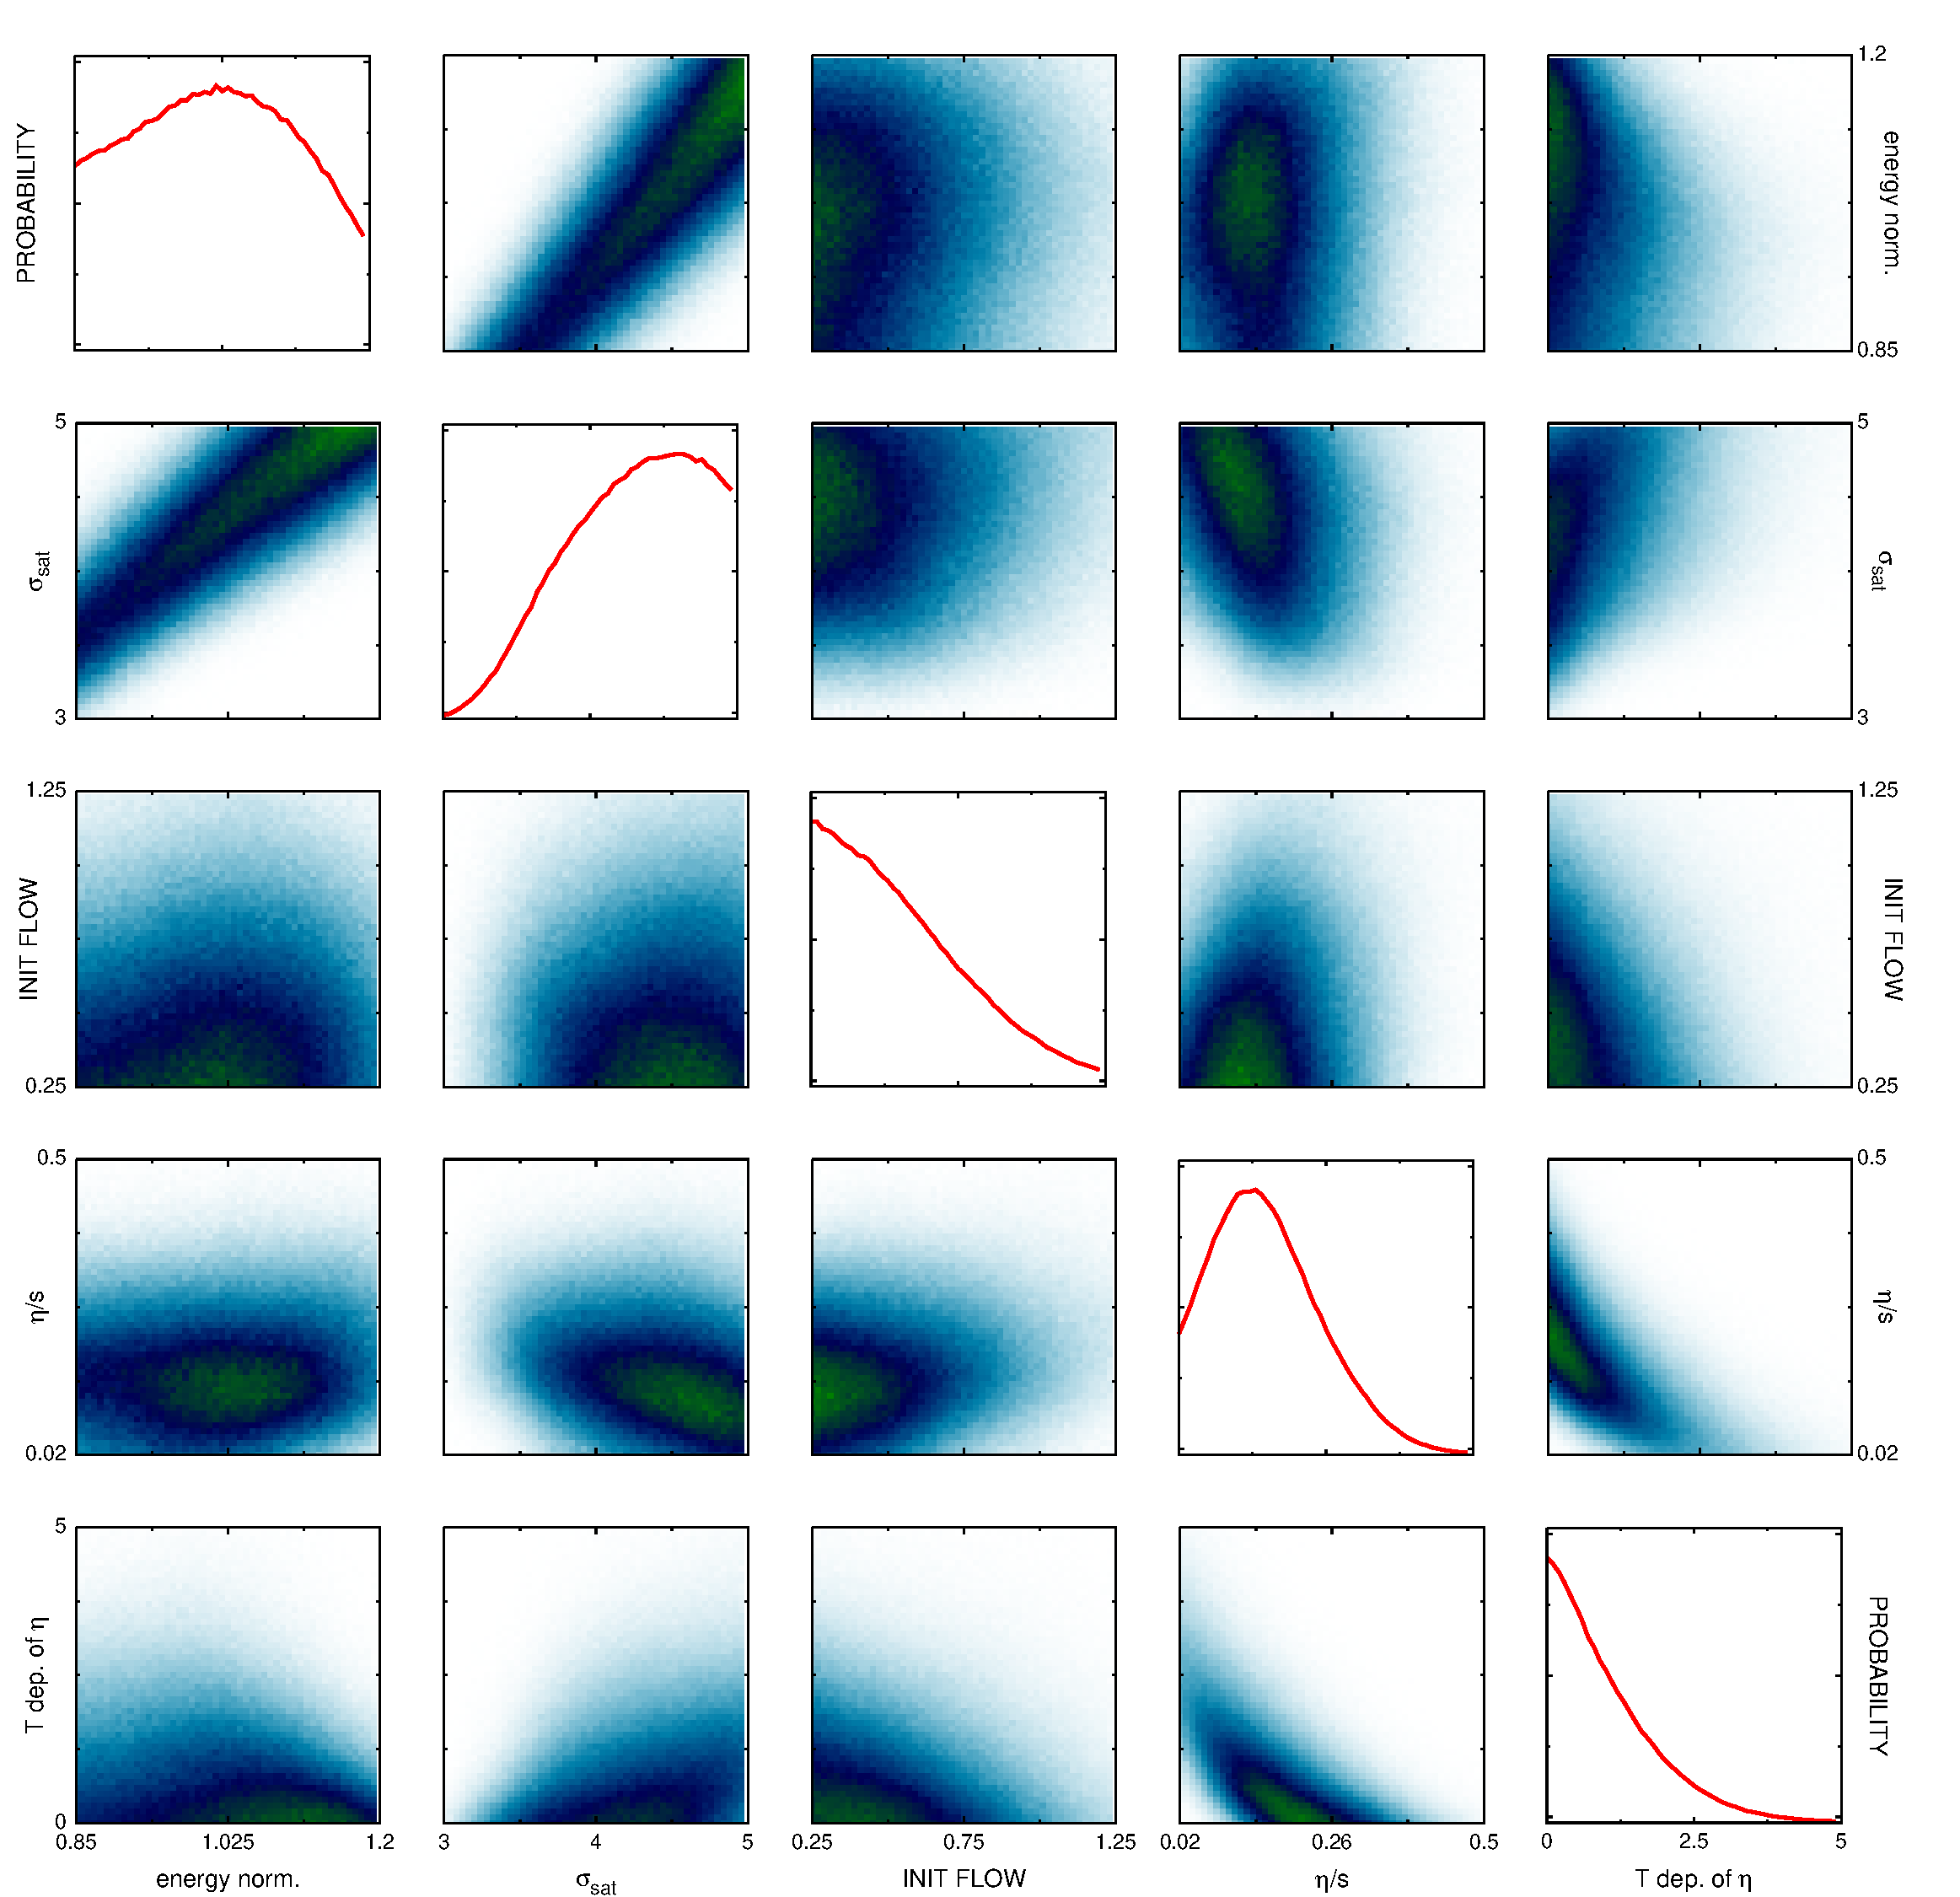
\includegraphics[width=0.8\textwidth]{figs/rhic.pdf}
\end{figure}
